\chapter{Question 2}
\label{question-2}
\section{Question}



\begin{itemize}
\item Using the pages from Q1 (A4), download all TimeMaps (including TimeMaps with 404 responses, i.e. empty or null TimeMaps)
\begin{itemize}
	\item Upload all the TimeMaps to github
\end{itemize}
\item Build a CDF for \# of mementos for each original URI (i.e., x-axis = \# of mementos, y-axis = \% of links)
\item See: \url{http://timetravel.mementoweb.org/guide/api/}
\end{itemize}

\section{Solution}

\begin{itemize}
\item For downloading the TimeMaps I modified my script from the first assignment to retrieve the html pages. I just had to add a prefix to the URL to include the memento aggregator URL. But I wasn't able to successfully download the TimeMaps for most of the files.
\item I then started using the script as provided in the mailing group by Alexander Nwala for retrieving the TimeMaps, but I noticed that the script was taking too long to run.
\item Soon after I got back to using my script with a modified memento aggregator URL to point to the following URL \url{http://labs.mementoweb.org/timemap/json/}. I was successfully able to retrieve in JSON format which would make my life simpler in processing the data.
\item Soon after I committed the TimeMaps to github.
\item I wrote a script to find the number of mementos in each of the URIs 
\end{itemize}

	\begin{minipage}{\linewidth}
		\centering
			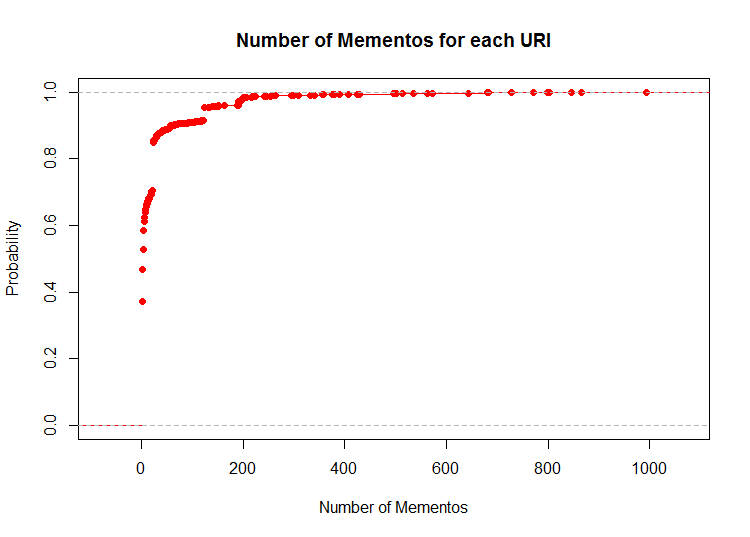
\includegraphics[scale=0.55]{figures/q2/numberMementos}
		\captionof{figure}{CDF - Number of Mementos for each URI}
		\label{wordCount}
	\end{minipage}
	

\newpage
\section{Code Listing}
\lstinputlisting[language=Python,breaklines = true,frame=single,caption={Python program for fetching the TimeMaps.},label=lst:q1-1,captionpos=b,numbers=left,showspaces=false,showstringspaces=false,basicstyle=\footnotesize]{pythonFiles/getTimeMap.py}
\newpage
\lstinputlisting[language=Python,breaklines = true,frame=single,caption={Python program for finding the number of mementos in each of the TimeMaps.},label=lst:q1-1,captionpos=b,numbers=left,showspaces=false,showstringspaces=false,basicstyle=\footnotesize]{pythonFiles/getMemento.py}

\newpage
\lstinputlisting[language=R,breaklines = true,frame=single,caption={R program for generating the CDF for number of mementos}, label=lst:q1R1,captionpos=b,numbers=left,showspaces=false,showstringspaces=false,basicstyle=\footnotesize]{rFiles/cdfQ2.r}